\section{Quadcopter Components}
When building a quadcopter, it is necessary to understand which parts that are necessary in the build and their purpose for the quadcopter.
The different parts of a quadcopter, are frame/chassis, motors, Propellers, Electronic speed controller (ESC), flight controller, battery, and if you want to remote control it, a radio system.

%
%
\subsection{Frame}
 The frame of the quadcopter is the skeleton that holds all part of the drone and comes in different shapes. The shapes that have the most notable characteristics, are the H-frame and X-frame.
 \newline
 \newline
The H-frame shape drone have a design that make more space to mount more modules on the drone. It also has the benefit of  having the battery mounted at the top of the quadcopter. With the battery mounted at the top of the quadcopter it insures that the quadcopter does not land on the battery and by this the battery are better protected \cite{FPVFrame}.
\newline
\newline
When taking about a H-frame, there are different style such as a true H-frame or a HX-frame, this can be seen in figure \ref{fig:QC_HFrame}. In figure \ref{fig:QC_TrueH-Frame} a true H-frame can be seen, and are as the name implies, a quadcopter frame that shape look like a H, where the HX-frame is a X shapes frame that has the central body of a H-frame and can be seen in figure \ref{fig:QC_HXFrame}.
\begin{figure}[h]
    \centering
    \begin{subfigure}[b]{0.49\textwidth}
        \centering
        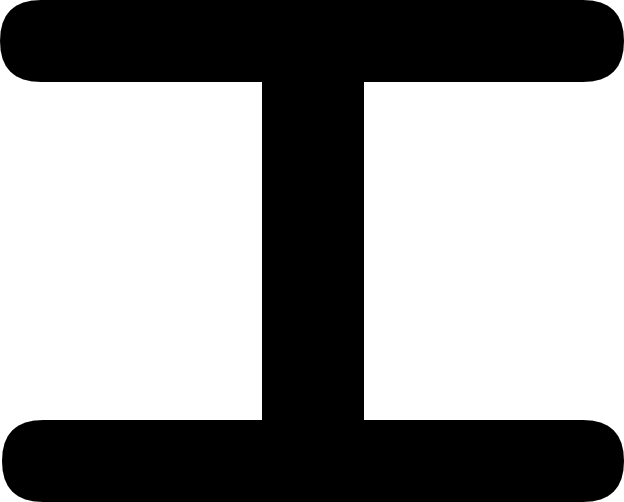
\includegraphics[width=0.5\textwidth]{figures/PA/QCComponent/H-shape.png}
        \caption{True H-shape frame}
        \label{fig:QC_TrueH-Frame}
    \end{subfigure}
    \begin{subfigure}[b]{0.49\textwidth}
        \centering
        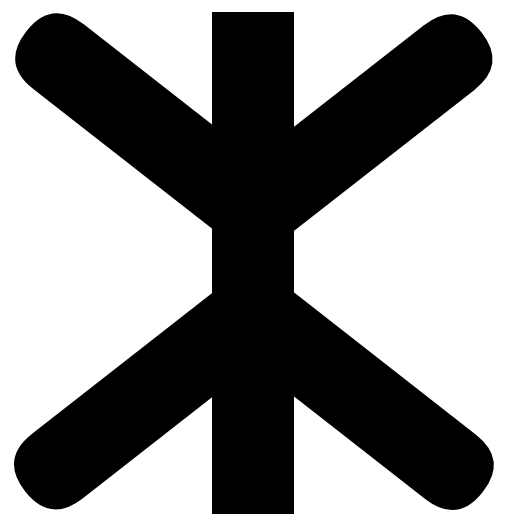
\includegraphics[width=0.5\textwidth]{figures/PA/QCComponent/HX-shape.png}
        \caption{HX-shape frame}
        \label{fig:QC_HXFrame}
    \end{subfigure}
    \caption{Two different style H-frame}
    \label{fig:QC_HFrame}
\end{figure}
\newline
The X-frame are a type of frame that, as the name implies, are a frame that has the shape of a X, as it can be seen in figure \ref{fig:QC_XFrame}. Because of the shape of the frame, there is less spaces to mount modules on, but this has the benefit of a lighter frame as is has no unnecessary weight. because the central body is smaller the battery will normally be mounted under the frame, which can damage the battery when landing, if landing on uneven terrain, with small feet.\cite{FPVFrame}.
\begin{figure}[h]
    \centering
    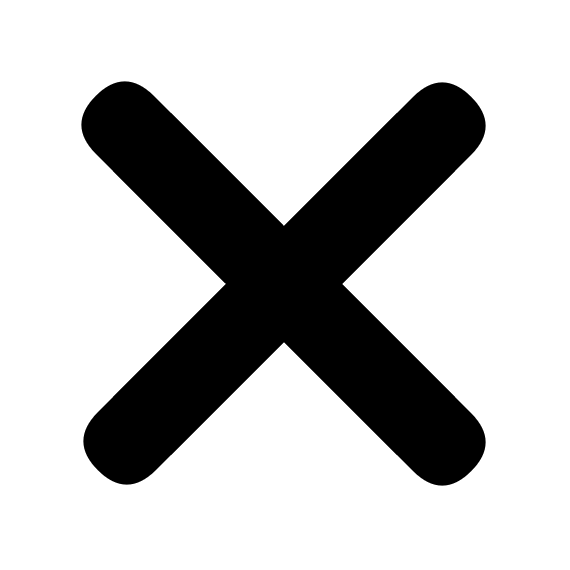
\includegraphics[width=0.3\textwidth]{figures/PA/QCComponent/X-shape_frame.png}
    \caption{X-shape frame}
    \label{fig:QC_XFrame}
\end{figure}
%
%
\subsection{Motors}
The next component a drone must use are motors, which are some of the more important components of the drone. The motors can be found in different types. The main motor type for drones would be Brushless DC Motors (BLDC), though brushed DC motors are also used on small drones. With BLDC motors for drones, there are two different variants Inrunners and outrunners. The inrunners are a type of motor, where it’s the outside of the motor that are still, and the rotor are in inside rotating. This type of motor has a higher rotation speed. The outrunner are the opposite of the inrunners as it’s the outside of the motor that’s rotating. This type is more common as it generates a higher torque to drive the propellers.
\newline
\newline
Motors are rated KV that stands for RPM per volt applied, which means that a higher KV will give a higher rotation speed \cite{DIYDrone}. Motors are also sold as clockwise and counter-clockwise, where a quadcopter needs 2 of each.

%
%
\subsection{Propellers}
The component that can have the highest effect on the thrust of the motors are the propellers. By increasing the size, more trust will be created at the same RPM, however more torque is also required. Thus, propeller size and motor rpm has to be matched. The measurements that the propellers are measured with are the diameter and the pitch. the diameter of the propeller is the length of them and are measured in inches.\\
The pitch of a propeller is the distance it would move in one rotation, if thought of as a screw. \cite{DIYDrone}.

%
%
\subsection{Electronic speed controller}
To control the speed of which the motors are spinning four electronic speed controllers or short ESC’s are used, one for each motor \cite{QuardcoptorParts}. 

On most RC vehicles, ESCs are 3-phase Variable Frequency Drives (VFD), as BLDC motors require 3 phase AC to be driven. 

When deciding which ESC that should be used of the quadcopter, the highest current draw of the motors is determined, and an ESC that has a value of it or higher is chosen \cite{DIYDrone}.

%
%
\subsection{Flight controller}
the brain of the quadcopter is the flight controller, which is a small computer that controls it. The flight controller has some in-build sensors such as gyroscopes and accelerometer to detect changes of the drone and control the motors, so the quadcopter stays in the air. the component that gets commands from the user are also the flight controller. A flight controller can also have inbuild barometric pressure sensors and magnetometer and are a hub so other components such as GPS or external sensors can be connected \cite{FlightController}.

%
%
\subsection{Battery}
The type of battery almost all quadcopters uses are LiPo batteries, as it has a high discharge rate. A problem with  using this type of battery is that they have are rather sensitive for overcharging and over-discharging. In these cases, hydrogen and heat is formed, which can lead to the battery 'puffing' or even bursting into flames.\\
Because of this, safety measures have to be taken when handling these batteries, especially when charging them as this is often a lengthy process, meaning it can't be fully supervised.\\
Some of the safety measures recommended when charging this type of battery, are to keep the them in a fire-safe bag when charging them, so if the battery burst in to flames the bag can contain it, and using a proper LiPo charger, not exceeding the max charging rate of the battery. 
\cite{DIYDrone}.

%
%
%\subsection{receiver transmitter} skal det med